

\documentclass[conference]{IEEEtran}

\usepackage[utf8]{inputenc}
\usepackage[T1]{fontenc}
\usepackage{lmodern} % load a font with all the characters
\usepackage{xcolor}
\usepackage{multicol}
\usepackage{graphicx}
\usepackage{subfig}
\usepackage{lipsum}
\usepackage{afterpage}
\graphicspath{ {images/} }
\newcommand\myworries[1]{\textcolor{red}{#1}}

% correct bad hyphenation here
\hyphenation{op-tical net-works semi-conduc-tor}


\begin{document}

\title{Trabalho de Algorítmos Genéticos\\ Parte 1}


\author{\IEEEauthorblockN{Fábio Beranizo Fontes Lopes}
\IEEEauthorblockA{Escola de Artes, Ciências e Humanidades (EACH)\\
Universidade de São Paulo (USP)\\
Email: f.lopes@usp.br}
}

% make the title area
\maketitle


\section{Introdução}
Este relatório apresenta a discussão da parte 1 do trabalho de algorítmos
genéticos (GA) para a disciplina de Inteligência Computacional. Foi avaliada a
utilização de GA para otimização de um conjunto funções. O foco se manteve em
analisar o comportamento do algorítmo mediante a utilização de
diferentes técnicas, operadores e parametrizações.\\
O trabalho foi desenvolvido utilizando a linguagem de programação Python,
especificamente sua distribuição Anaconda.\\


\section{Otimização de Funções}
O problema da otimização de funções consiste em maximizar ou minimizar uma 
função matemática através da escolha de valores para as variáveis,
respeitando-se o domínio da função.
Para o trabalho desenvolvido foram selecionadas 4 funções para análise:

\[max. f_0(x) = 20 + \sum_{i=1}^{2} x_{i}^{2} - 10\cos(2\pi x_i)\]
\begin{center}intervalo para otimização: [-5, 5]\\\end{center}

\[min. f_1(x) = \sum_{i=1}^{30} x_{i}^{2}\]
\begin{center}intervalo para otimização: [-100, 100]\\\end{center}

\[min. f_2(x) = \sum_{i=1}^{30} \left|x_i + 0.5\right|^{2}\]
\begin{center}intervalo para otimização: [-100, 100]\\\end{center}

\[min. f_3(x) = \sum_{i=1}^{30} -x_i \sin(\sqrt(\left|x_i\right|))\]
\begin{center}intervalo para otimização: [-500, 500]\\\end{center}

Para facilitar a implementação as funções para minimização foram transformadas 
no oposto e maximizadas.

\section{Cromossomo}
Para a representação de uma solução do problema de otimização de funções foi
necessário utilizar uma estrutura que armazenasse o valor das variáveis da
solução. A escolha natural foi adotar vetores como estrutura de dados. Essa
decisão facilitou a implementação dos operadores de crossover e de mutação, além
de tornar simples o cálculo das funções fitness.
Cada variável da solução podia assumir um valor real dentro de um domínio. Para
dispor as variáveis dentro do vetor foram realizadas duas abordagens, cromossomo
de valores reais e cromossomo de valores binários.\\

\subsection{Cromossomo Real}
No cromossomo real cada elemento do vetor assume um valor \textit{float} que
representa o valor da variável. O genótipo do indivíduo é do tipo:
\[[float_{var_1}, float_{var_2}, ..., float_{var_n}]\]

\subsection{Cromossomo Binário}
No cromossomo binário cada elemento do vetor representa um bit de uma das 
variáveis da solução. Cada variável ocupa 32 bits contínuos, ou seja, 32 
posições do vetor de um indivíduo. O genótipo do indivíduo é do tipo:

\[[bit1_{var_1}, bit2_{var_1}, ..., bit32_{var_n}]\]\\

Na seção de discussão dos resultados serão avaliadas as vantagens e desvantagens
de cada abordagem de cromossomo.

\section{Seleção de Indivíduos}
Somente um operador de seleção de indivíduos foi analisado neste trabalho, o
método da roleta. Ele operador foi escolhido por ser de fácil implementação e
por apresentar bons resultados segundo a literatura. No entanto, durante o
desenvolvimento foi possível perceber um problema: este operador aumenta
consideravelmente o tempo de execução do algorítmo para grandes populações, uma 
vez que todos os indivíduos participam do sorteio.

\subsection{Método da Roleta}
O método da roleta leva em consideração o fitness de um indivíduo em relação ao
fitness total da população. Nesse processo cada indivíduo possui uma 
probabilidade de ser selecionado (uma fatia da roleta) proporcional ao seu
fitness. Embora não garanta que as melhores soluções sobrevivam, este método
dá mairoes probabilidades de sobrevida às soluções com bom fitness.

\section{Operadores Genéticos}
Os indivíduos selecionados passam por um dos 3 tipos principais de operadores
genéticos: reprodução, crossover e mutação. Neste trabalho foram analisados
dois tipos de crossover e dois tipos de mutação, que são descritos abaixo:\\

\subsection{Crossover}
O operador crossover permite a criação de novos indivíduos a partir de
organismos pais. Os descendentes possuem genótipo de ambos pais, embora
geralmente sejam diferentes. O crossover é uma forma de ampliar o espaço de
busca por soluções, porém mantendo-se material genético de boa qualidade de
gerações anteriores.

\subsubsection{Crossover de um Ponto}
O crossover de um ponto seleciona aleatoriamente um ponto de crossover nos
cromossomos pais e os recombina gerando dois filhos. Este operador favorece a
herança de trechos contínuos de cromossomo, o que pode ser bom quando estes
trechos guardam algum significado para o fitness.

\subsubsection{Crossover Uniforme}
O crossover uniforme define cada gene de um novo indivíduo copiando-se o valor
de um de seus pais com uma dada probabilidade. Essa abordagem, ao contrário do
crossover de um ponto, quebra trechos contínuos de cromossomo e podendo levar a
uma maior diversidade do espaço de busca.

\subsection{Mutação}
O operador de mutação permite inserir diversidade genética entre gerações de
indivíduos trocando o valor de genes no cromossomo. Com maior variedade genética
o espaço de busca é ampliado, permitindo sair de situações de mínimo local.
Entretanto, os experimentos realizados indicaram que este operador deve ser
usado com parcimônia, com baixa probabilidade de ocorrer. Nas parametrizações em
que sua probabilidade foi alta a busca não convergiu para bons valores, mantendo
quase um comportamento de busca aleatória.

\subsubsection{Mutação Simples}
A operação de mutação básica consiste em sortear uma posição do cromossomo e
substituí-la por um valor aleatório do domínio da solução. Essa operação deve
manter a solução válida, evitando-se processamento para verificação do
cromossomo.

\subsubsection{Mutação por Permutação}
Outro operador avaliado foi a mutação por permutação. Neste tipo de mutação,
dois genes do cromossomo são sorteados e trocam de posição entre si. Este tipo
de mutação não causou impacto no cromossomo real, uma vez que nas funções
avaliadas as variáveis tinham o mesmo peso. No entanto, para o cromossomo
binário essa técnica é interessante pois promove mudança significativa dos
genes e é executada mais rapidamente que a mutação simples.

\section{Elitismo}
Em algorítmos genéticos o elitismo é a operação de copiar uma dada proporção dos
melhores indivíduos para a próxima geração. Esta técnica garante que boas 
soluções permaneçam na população, evitando-se que o algorítmo deixe de explorar 
espaços de busca promissores.
Na solução desenvolvida elitismo foi implementado conservando 10\% dos
indivíduos com melhor fitness da geração anterior.

\section{Critério de Parada}
A evolução do algorítmo genético prossegue até que que um critério de parada
seja atingido. Neste trabalho foram comparados 2 alternativas para término da
evolução: número de gerações e tempo de execução. Ambas técnicas não são
sofisticadas, nem são ótimas do ponto de vista de resultados, no entanto
permitem realizar uma análise mais adequada dos operadores. Comparando-se
diferentes parametrizações mediante um mesmo tempo de execução, ou um
determinado número de gerações é possível avaliar de forma justa as vantagens e
desvantagens de cada escolha.

\subsection{Número de Gerações}
Este critério de parada de faz o com o algorítmo prossiga até que um determinado
número de gerações seja atingido. Dessa forma é possível comparar quais
parametrizações convergem mais rapidamente, além de avaliar o quanto são
propensas a ficar presas em mínimos locais.

\subsection{Tempo de Execução}
No segundo critério avaliado é dado um tempo limite para a execução do
algorítmo. Este critério é interessante para avaliar quais técnicas são mais
custosas do ponto de vista de processamento, e quais se sairiam melhor em 
situação de restrição do tempo disponível. Nos testes realizados foi fixado 
1 segundo para evolução em cada parametrização.

\section{Grid Search}
O resultado da execução do algorítmo genético está ligado diretamente aos
parâmetros utilizados. Tais parâmetros podem ser selecionados eficientemente
através de uma busca de parametrizações geradas a partir de um \textit{grid}.
Este processo é denominado \textit{Grid Search}.\\
Para o algorítmo genético desenvolvido, os parâmetros otimizados foram: tamanho 
da população de indivíduos e probabilidades dos operadores de reprodução, 
crossover e mutação.

\begin{figure*}[!t]
\centering
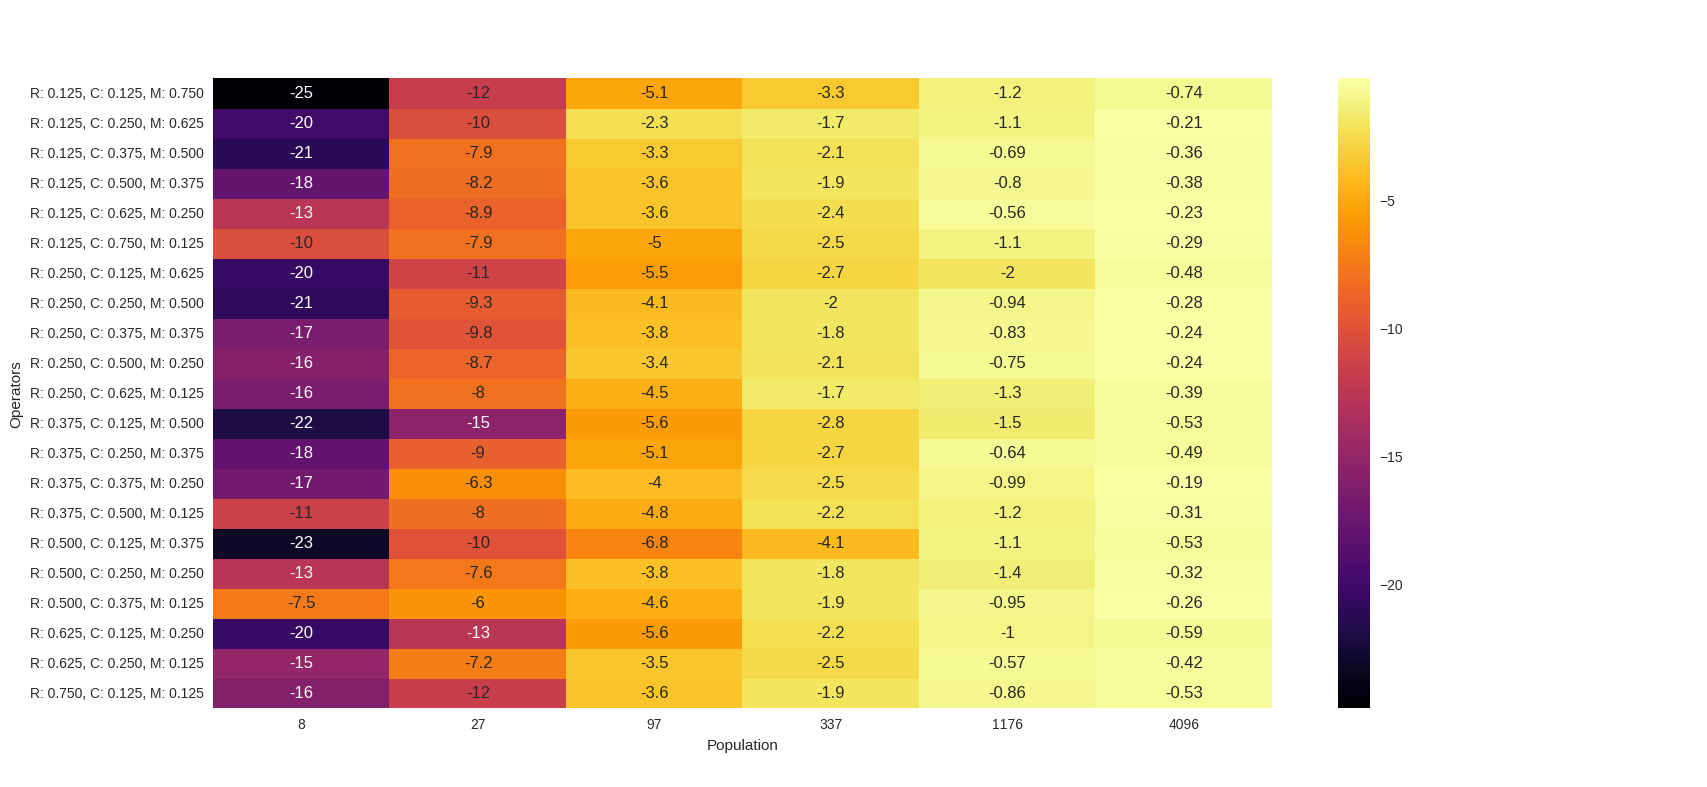
\includegraphics[scale=0.5]{f0_test_grid_search_100_generations}
\caption{Resultados do Grid Search para f0(x) e 100 gerações}
\end{figure*}

\begin{figure*}[!t]
\centering
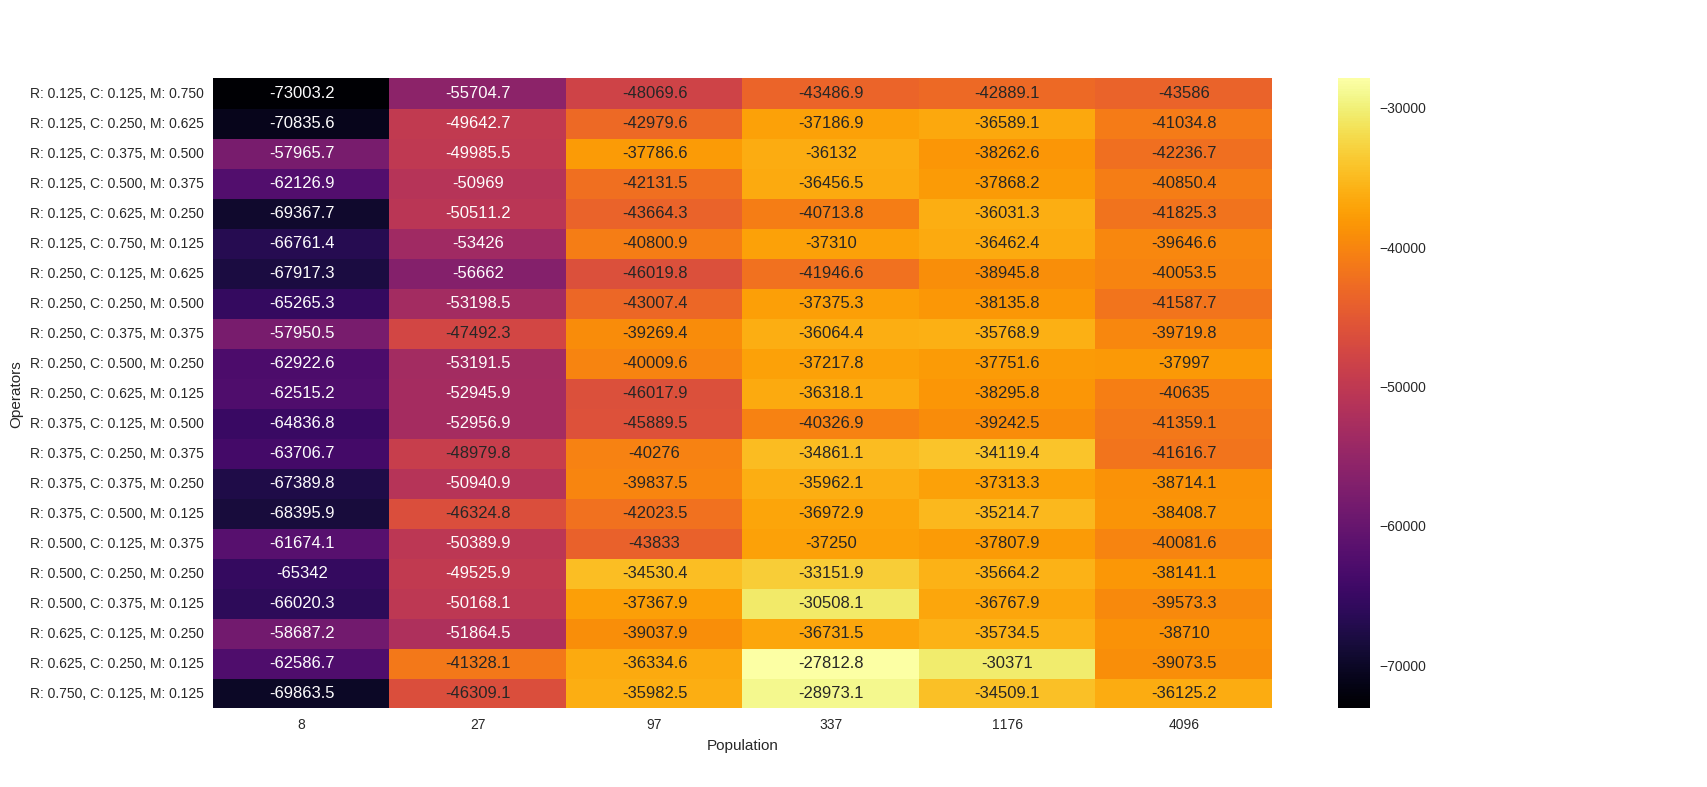
\includegraphics[scale=0.5]{f2_test_grid_search_1_second}
\caption{Resultados do Grid Search para f2(x) e 1 segundo de execução}
\end{figure*}


\subsection{Parâmetros Variados}
Visando avaliar o comportamento do algorítmo com populações de tamanhos bem 
distintos, foram testadas 6 possíveis variações de população: de 8 a 4096
indivíduos dispostos em escala logarítimica.\\
As probabilidades dos operadores foram variadas de 0.125 a 0.875 em espaços de 
0.125.\\
Arbitrariamente foi definido que a escolha da melhor parametrização seria feita 
utilizando uma configuração base de operadores. Após definida a melhor escolha 
de parâmetros, os mesmos foram aplicados para outros tipos de operadores, técnicas e 
cromossomo, e uma análise comparativa foi realizada.

Configuração base de operadores:
\begin{itemize}
\item Cromossomo real
\item Crossover de um ponto
\item Mutação simples
\item Não há elitismo
\end{itemize}

Para que os resultados do do \textit{Grid Search} fossem mais confiáveis, cada
parametrização foi executada 10 vezes. A média dos melhores fitness obtidos nas
10 execuções foram então dispostas nos gráficos abaixo para avaliação:

Observando-se as figuras 1 e 2 é possível elaborar uma hipótese que há relação direta
entre o tamanho da população e a convergência do algorítmo para melhores valores.
De fato, em todos os testes executados, as parametrizações com maior população
alcançaram melhores resultados. A explicação para este fenômeno é que em
populações maiores a diversidade genética é maior e consequentemente o espaço de
busca também. Mesmo no caso da figura 2 em que o tempo de execução para todas
parametrizações é o mesmo, a população se mostrou mais determinante para obter
bons resultados que o tempo de execução do algorítmo.\\
Há no entanto uma ressalva: embora populações maiores contribuam para bons 
resultados, o tempo de execução do algorítimo é fortemente impactado por este 
grande número de indivíduos. Dependendo da aplicação isso deve ser levado em 
consideração.\\

Para as comparações foram fixados os seguintes parâmetros:
\begin{itemize}
\item Taxa de reprodução = 0.375
\item Taxa de crossover = 0.500
\item Taxa de mutação = 0.125
\item Tamanho da população = 27
\end{itemize}

O tamanho da população foi propositalmente mantido não muito grande para que o 
resultado pudesse convergir mais lentamente.

\section{Operadores e Estratégias}
Dada a parametrização definida anteriormente, foram avaliados a seguir 
diferentes operadores e estratégias genéticas.

\subsection{Elitismo}
A Figura 3 mostra uma comparação das evoluções com e sem elitismo. Analisando os
resultados é possível perceber que a solução com elitismo evita a perda da melhor 
solução, que ocorre na versão sem elitismo. Além disso, a aplicação desta técnica
permitiu que a solução convergisse para melhores valores mais rapidamente.

A tabela 1 mostra valores de fitness obtidos em execuções do algorítmo
com e sem elitismo:\\


\begin{table}[h]
\begin{tabular}{|l|l|l|}
\hline
      & Fit max s/ Elitismo & Fit max c/ Elitismo \\ \hline
f0(x) & -1.0656             & -1.91               \\ \hline
f1(x) & -42369.4015         & -27148.6555         \\ \hline
f2(x) & -49484.2555         & -25797.7171         \\ \hline
f3(x) & 3172.7526           & 6228.4944           \\ \hline
\end{tabular}
\caption*{Tabela 1 - Valores de fitness para evolução c/ e s/ elitismo}
\end{table}


\begin{figure*}[!t]
\centering
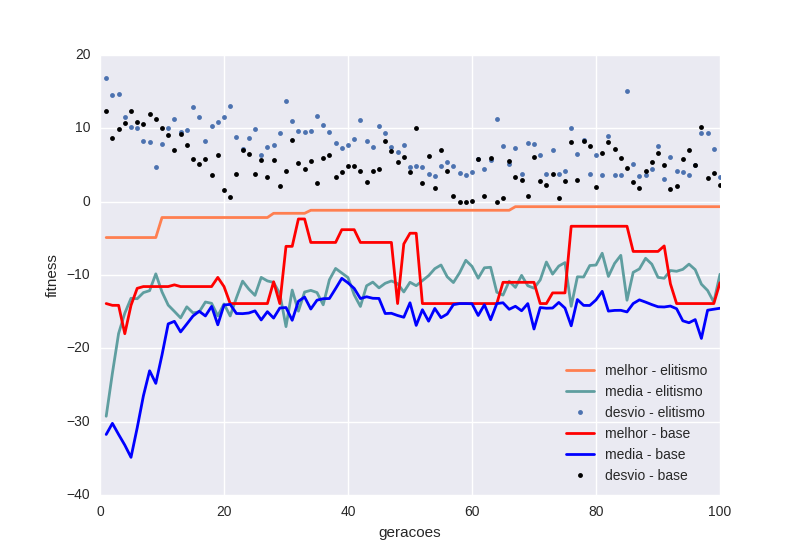
\includegraphics[scale=0.5]{f0_elitism}
\caption{Evolução do algorítimo genético c/ e s/ elitismo}
\end{figure*}

\subsection{Operadores de Crossover}
O resultado dos operadores de crossover foi parelho nos testes. A tabela 2
mostra que para as funções f0 e f1 o crossover de um ponto obteve fitness 
melhores e para f2 e f3 o crossover uniforme foi superior. \\
De fato, para o cromossomo real nenhum dos operadores escolhidos possui alguma 
vantagem uma vez que não há esquemas, nem sequências especiamente importantes.\\

\begin{table}[]
\begin{tabular}{|l|l|l|}
\hline
      & Fit max C. um ponto & Fit max C. uniforme \\ \hline
f0(x) & -1.0656             & -2.2871             \\ \hline
f1(x) & -42369.4015         & -66625.7284         \\ \hline
f2(x) & -49484.2555         & -42732.2830         \\ \hline
f3(x) & 3172.7526           & 3166.0494           \\ \hline
\end{tabular}
\caption*{Tabela 2 - Valores de fitness para evolução c/ crossover de um ponto e uniforme}
\end{table}

\subsection{Operadores de Mutação}
A Figura 8 mostra a comparação das evoluções dos operadores de mutação básica e
por permutação. Observando-se os resultados, claramente a mutação simples levou 
a melhores fitness nas execuções. Conforme discutido anteriormente, este 
resultado se deve ao fato da Mutação por permutação não alterar o resultado da 
função fitness para cromossomos reais.\\

\begin{table}[]
\begin{tabular}{|l|l|l|}
\hline
      & Fit max C. um ponto & Fit max C. uniforme \\ \hline
f0(x) & -1.0656             & -9.1838             \\ \hline
f1(x) & -42369.4015         & -56952.5563         \\ \hline
f2(x) & -49484.2555         & -55968.1716         \\ \hline
f3(x) & 3172.7526           & 2487.9347           \\ \hline
\end{tabular}
\caption*{Tabela 3 - Valores de fitness para evolução c/ mutação simples e permutação}
\end{table}


\subsection{Cromossomo Binário}
O cromossomo binário foi implementado, porém os resultados não foram totalmente 
analisados devido a problemas nos testes executados. 
No entanto, é possível supor que sua característica poderia levar a convergência
exata para o ótimo nas funções f0, f1 e f2, cujo máximo global é zero.
Além disso, o uso do operador de permutação se tornaria mais relevante,
inserindo variedade genética para a função avaliada.
O operador de crossover uniforme por sua vez se comportaria como quase que uma 
mutação, uma vez que modificaria significantemente a composição dos valores das 
variáveis.

% An example of a floating figure using the graphicx package.
% Note that \label must occur AFTER (or within) \caption.
% For figures, \caption should occur after the \includegraphics.
% Note that IEEEtran v1.7 and later has special internal code that
% is designed to preserve the operation of \label within \caption
% even when the captionsoff option is in effect. However, because
% of issues like this, it may be the safest practice to put all your
% \label just after \caption rather than within \caption{}.
%
% Reminder: the "draftcls" or "draftclsnofoot", not "draft", class
% option should be used if it is desired that the figures are to be
% displayed while in draft mode.
%
%\begin{figure}[!t]
%\centering
%\includegraphics[width=2.5in]{myfigure}
% where an .eps filename suffix will be assumed under latex, 
% and a .pdf suffix will be assumed for pdflatex; or what has been declared
% via \DeclareGraphicsExtensions.
%\caption{Simulation results for the network.}
%\label{fig_sim}
%\end{figure}

% Note that the IEEE typically puts floats only at the top, even when this
% results in a large percentage of a column being occupied by floats.


% An example of a double column floating figure using two subfigures.
% (The subfig.sty package must be loaded for this to work.)
% The subfigure \label commands are set within each subfloat command,
% and the \label for the overall figure must come after \caption.
% \hfil is used as a separator to get equal spacing.
% Watch out that the combined width of all the subfigures on a 
% line do not exceed the text width or a line break will occur.
%
%\begin{figure*}[!t]
%\centering
%\subfloat[Case I]{\includegraphics[width=2.5in]{box}%
%\label{fig_first_case}}
%\hfil
%\subfloat[Case II]{\includegraphics[width=2.5in]{box}%
%\label{fig_second_case}}
%\caption{Simulation results for the network.}
%\label{fig_sim}
%\end{figure*}
%
% Note that often IEEE papers with subfigures do not employ subfigure
% captions (using the optional argument to \subfloat[]), but instead will
% reference/describe all of them (a), (b), etc., within the main caption.
% Be aware that for subfig.sty to generate the (a), (b), etc., subfigure
% labels, the optional argument to \subfloat must be present. If a
% subcaption is not desired, just leave its contents blank,
% e.g., \subfloat[].


% An example of a floating table. Note that, for IEEE style tables, the
% \caption command should come BEFORE the table and, given that table
% captions serve much like titles, are usually capitalized except for words
% such as a, an, and, as, at, but, by, for, in, nor, of, on, or, the, to
% and up, which are usually not capitalized unless they are the first or
% last word of the caption. Table text will default to \footnotesize as
% the IEEE normally uses this smaller font for tables.
% The \label must come after \caption as always.
%
%\begin{table}[!t]
%% increase table row spacing, adjust to taste
%\renewcommand{\arraystretch}{1.3}
% if using array.sty, it might be a good idea to tweak the value of
% \extrarowheight as needed to properly center the text within the cells
%\caption{An Example of a Table}
%\label{table_example}
%\centering
%% Some packages, such as MDW tools, offer better commands for making tables
%% than the plain LaTeX2e tabular which is used here.
%\begin{tabular}{|c||c|}
%\hline
%One & Two\\
%\hline
%Three & Four\\
%\hline
%\end{tabular}
%\end{table}


% Note that the IEEE does not put floats in the very first column
% - or typically anywhere on the first page for that matter. Also,
% in-text middle ("here") positioning is typically not used, but it
% is allowed and encouraged for Computer Society conferences (but
% not Computer Society journals). Most IEEE journals/conferences use
% top floats exclusively. 
% Note that, LaTeX2e, unlike IEEE journals/conferences, places
% footnotes above bottom floats. This can be corrected via the
% \fnbelowfloat command of the stfloats package.


% conference papers do not normally have an appendix

% use section* for acknowledgment




% trigger a \newpage just before the given reference
% number - used to balance the columns on the last page
% adjust value as needed - may need to be readjusted if
% the document is modified later
%\IEEEtriggeratref{8}
% The "triggered" command can be changed if desired:
%\IEEEtriggercmd{\enlargethispage{-5in}}

% references section

% can use a bibliography generated by BibTeX as a .bbl file
% BibTeX documentation can be easily obtained at:
% http://mirror.ctan.org/biblio/bibtex/contrib/doc/
% The IEEEtran BibTeX style support page is at:
% http://www.michaelshell.org/tex/ieeetran/bibtex/
%\bibliographystyle{IEEEtran}
% argument is your BibTeX string definitions and bibliography database(s)
%\bibliography{IEEEabrv,../bib/paper}
%
% <OR> manually copy in the resultant .bbl file
% set second argument of \begin to the number of references
% (used to reserve space for the reference number labels box)
\begin{thebibliography}{1}

\bibitem{}
S. Peres, Buscas - Inteligência Artificial, Apresentação realizada durante a disciplina SIN5002. 10 mar 2016.


\bibitem{}
S. Russell and P. Norvig, Artificial intelligence. Englewood Cliffs, N.J.: Prentice Hall, 1995.

\end{thebibliography}




% that's all folks
\end{document}


